% Created by tikzDevice version 0.8.1 on 2015-01-07 14:23:30
% !TEX encoding = UTF-8 Unicode
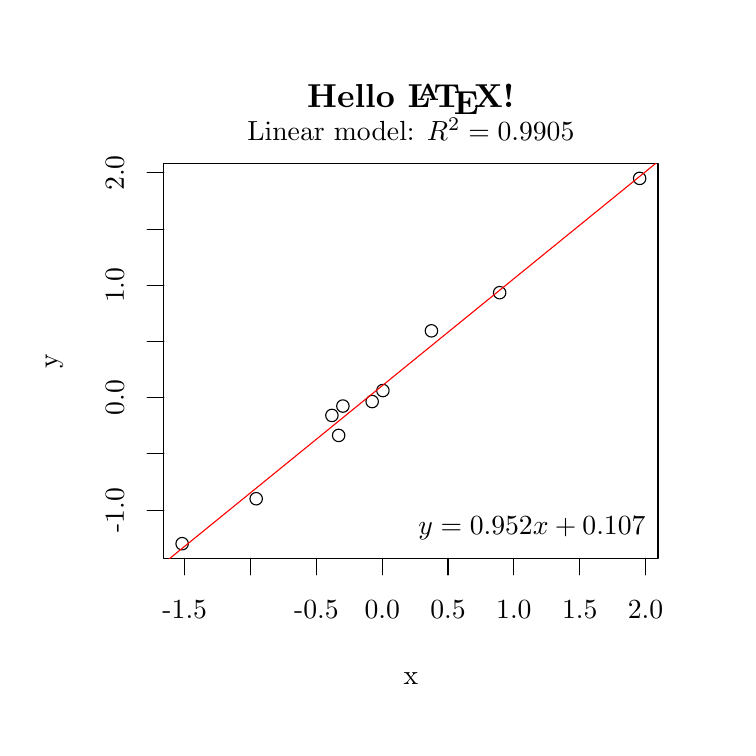
\begin{tikzpicture}[x=1pt,y=1pt]
\definecolor{fillColor}{RGB}{255,255,255}
\path[use as bounding box,fill=fillColor,fill opacity=0.00] (0,0) rectangle (252.94,252.94);
\begin{scope}
\path[clip] ( 49.20, 61.20) rectangle (227.75,203.75);
\definecolor{drawColor}{RGB}{0,0,0}

\path[draw=drawColor,line width= 0.4pt,line join=round,line cap=round] (128.36,121.82) circle (  2.25);

\path[draw=drawColor,line width= 0.4pt,line join=round,line cap=round] ( 55.81, 66.48) circle (  2.25);

\path[draw=drawColor,line width= 0.4pt,line join=round,line cap=round] (109.93,112.82) circle (  2.25);

\path[draw=drawColor,line width= 0.4pt,line join=round,line cap=round] (170.55,157.18) circle (  2.25);

\path[draw=drawColor,line width= 0.4pt,line join=round,line cap=round] (112.37,105.60) circle (  2.25);

\path[draw=drawColor,line width= 0.4pt,line join=round,line cap=round] ( 82.57, 82.72) circle (  2.25);

\path[draw=drawColor,line width= 0.4pt,line join=round,line cap=round] (145.90,143.39) circle (  2.25);

\path[draw=drawColor,line width= 0.4pt,line join=round,line cap=round] (113.90,116.21) circle (  2.25);

\path[draw=drawColor,line width= 0.4pt,line join=round,line cap=round] (124.48,117.84) circle (  2.25);

\path[draw=drawColor,line width= 0.4pt,line join=round,line cap=round] (221.13,198.47) circle (  2.25);
\end{scope}
\begin{scope}
\path[clip] (  0.00,  0.00) rectangle (252.94,252.94);
\definecolor{drawColor}{RGB}{0,0,0}

\path[draw=drawColor,line width= 0.4pt,line join=round,line cap=round] ( 56.77, 61.20) -- (223.25, 61.20);

\path[draw=drawColor,line width= 0.4pt,line join=round,line cap=round] ( 56.77, 61.20) -- ( 56.77, 55.20);

\path[draw=drawColor,line width= 0.4pt,line join=round,line cap=round] ( 80.56, 61.20) -- ( 80.56, 55.20);

\path[draw=drawColor,line width= 0.4pt,line join=round,line cap=round] (104.34, 61.20) -- (104.34, 55.20);

\path[draw=drawColor,line width= 0.4pt,line join=round,line cap=round] (128.12, 61.20) -- (128.12, 55.20);

\path[draw=drawColor,line width= 0.4pt,line join=round,line cap=round] (151.90, 61.20) -- (151.90, 55.20);

\path[draw=drawColor,line width= 0.4pt,line join=round,line cap=round] (175.68, 61.20) -- (175.68, 55.20);

\path[draw=drawColor,line width= 0.4pt,line join=round,line cap=round] (199.47, 61.20) -- (199.47, 55.20);

\path[draw=drawColor,line width= 0.4pt,line join=round,line cap=round] (223.25, 61.20) -- (223.25, 55.20);

\node[text=drawColor,anchor=base,inner sep=0pt, outer sep=0pt, scale=  1.00] at ( 56.77, 39.60) {-1.5};

\node[text=drawColor,anchor=base,inner sep=0pt, outer sep=0pt, scale=  1.00] at (104.34, 39.60) {-0.5};

\node[text=drawColor,anchor=base,inner sep=0pt, outer sep=0pt, scale=  1.00] at (128.12, 39.60) {0.0};

\node[text=drawColor,anchor=base,inner sep=0pt, outer sep=0pt, scale=  1.00] at (151.90, 39.60) {0.5};

\node[text=drawColor,anchor=base,inner sep=0pt, outer sep=0pt, scale=  1.00] at (175.68, 39.60) {1.0};

\node[text=drawColor,anchor=base,inner sep=0pt, outer sep=0pt, scale=  1.00] at (199.47, 39.60) {1.5};

\node[text=drawColor,anchor=base,inner sep=0pt, outer sep=0pt, scale=  1.00] at (223.25, 39.60) {2.0};

\path[draw=drawColor,line width= 0.4pt,line join=round,line cap=round] ( 49.20, 78.62) -- ( 49.20,200.46);

\path[draw=drawColor,line width= 0.4pt,line join=round,line cap=round] ( 49.20, 78.62) -- ( 43.20, 78.62);

\path[draw=drawColor,line width= 0.4pt,line join=round,line cap=round] ( 49.20, 98.93) -- ( 43.20, 98.93);

\path[draw=drawColor,line width= 0.4pt,line join=round,line cap=round] ( 49.20,119.24) -- ( 43.20,119.24);

\path[draw=drawColor,line width= 0.4pt,line join=round,line cap=round] ( 49.20,139.54) -- ( 43.20,139.54);

\path[draw=drawColor,line width= 0.4pt,line join=round,line cap=round] ( 49.20,159.85) -- ( 43.20,159.85);

\path[draw=drawColor,line width= 0.4pt,line join=round,line cap=round] ( 49.20,180.15) -- ( 43.20,180.15);

\path[draw=drawColor,line width= 0.4pt,line join=round,line cap=round] ( 49.20,200.46) -- ( 43.20,200.46);

\node[text=drawColor,rotate= 90.00,anchor=base,inner sep=0pt, outer sep=0pt, scale=  1.00] at ( 34.80, 78.62) {-1.0};

\node[text=drawColor,rotate= 90.00,anchor=base,inner sep=0pt, outer sep=0pt, scale=  1.00] at ( 34.80,119.24) {0.0};

\node[text=drawColor,rotate= 90.00,anchor=base,inner sep=0pt, outer sep=0pt, scale=  1.00] at ( 34.80,159.85) {1.0};

\node[text=drawColor,rotate= 90.00,anchor=base,inner sep=0pt, outer sep=0pt, scale=  1.00] at ( 34.80,200.46) {2.0};

\path[draw=drawColor,line width= 0.4pt,line join=round,line cap=round] ( 49.20, 61.20) --
	(227.75, 61.20) --
	(227.75,203.75) --
	( 49.20,203.75) --
	( 49.20, 61.20);
\end{scope}
\begin{scope}
\path[clip] (  0.00,  0.00) rectangle (252.94,252.94);
\definecolor{drawColor}{RGB}{0,0,0}

\node[text=drawColor,anchor=base,inner sep=0pt, outer sep=0pt, scale=  1.20] at (138.47,224.20) {\bfseries Hello \LaTeX!};

\node[text=drawColor,anchor=base,inner sep=0pt, outer sep=0pt, scale=  1.00] at (138.47, 15.60) {x};

\node[text=drawColor,rotate= 90.00,anchor=base,inner sep=0pt, outer sep=0pt, scale=  1.00] at ( 10.80,132.47) {y};
\end{scope}
\begin{scope}
\path[clip] ( 49.20, 61.20) rectangle (227.75,203.75);
\definecolor{drawColor}{RGB}{255,0,0}

\path[draw=drawColor,line width= 0.4pt,line join=round,line cap=round] ( 49.20, 59.41) -- (227.75,204.56);
\end{scope}
\begin{scope}
\path[clip] (  0.00,  0.00) rectangle (252.94,252.94);
\definecolor{drawColor}{RGB}{0,0,0}

\node[text=drawColor,anchor=base,inner sep=0pt, outer sep=0pt, scale=  1.00] at (138.47,212.14) {Linear model: $R^{2}= 0.9905 $};
\end{scope}
\begin{scope}
\path[clip] ( 49.20, 61.20) rectangle (227.75,203.75);
\definecolor{drawColor}{RGB}{0,0,0}

\node[text=drawColor,anchor=base west,inner sep=0pt, outer sep=0pt, scale=  1.00] at (141.16, 69.76) {$y = 0.952x +0.107$};
\end{scope}
\end{tikzpicture}
